\chapter{Introduction}\label{chp:introduction}

\todo{Write stuff as introduction. Or not. Is it needed?}

The goal of this project is to maximize user utility in video conference solutions. To maximize utility, we need to have a well-defined sense of what that implies.

\section{Context and utility}

When defining user utility, context is everything. You have different expectations to audiovisual quality on a desktop computer with fiber connectivity compared to your phone on 3G. But how can this difference be quantized? Certainly it's not a question of screen resolution, as most smart phones today have the same 1080p resolution as most computer screens. Resolutions beyond 1080p like we can find on some "retina" screens are not that interesting for video conferencing, as the webcam producing the source video is unlikely to be able to match that.

However, physical screen size matters. Viewing distance matters. Latency matters very much. Bandwidth matters. Packet loss matters. Most of these should be fairly easy to estimate, but then we have a new problem: which of these attributes do we prioritize? Finding the optimal balance is the key to optimizing user utility. There are of course also non-technical factors that affects the expected experience quite much that cannot be determined by the device itself. For example, even though the device is the same, you'll have different expectations sitting on the bus to work compared to sitting in a sofa in your living room, even though the device is the same. Environment matters. Mood matters. Time of day probably matters. We will however not take all of these factors into account, but limit our scope to the device itself, and since the intended application is to WebRTC, what we can relatively easy determine through the browser.

There will also be diminishing returns on most of these metrics. If you have practically unlimited bandwidth available, there's little to gain from sending video with bitrates in excess of 3 Mbps, you'll just be wasting bandwidth, CPU and battery. If we define a quality threshold for a device as the "optimal" experience that can be attained as 1.0, there's no reason to try to push this as high as possible. We can though assume that all metrics that are lower than what's necessary for this optimal experience will subtract from this quality metric somehow. For example, if we say that the threshold for optimal latency for a device is \(20ms\), we can imagine a \gls{utility function} that behaves like \(arctan(c-x)\), like illustrated in \autoref{fig:utility-latency}.

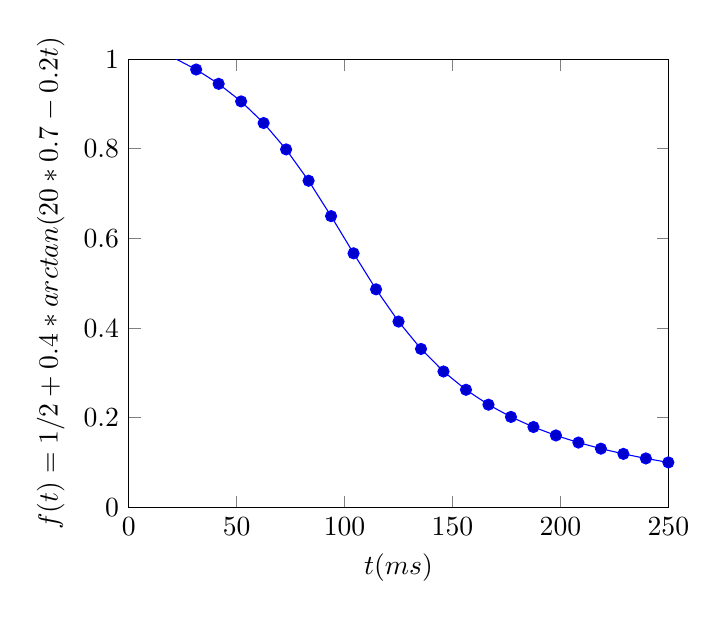
\begin{tikzpicture}
    \begin{axis}[
        xlabel={$t (ms)$},
        ylabel={$f(t) = 1/2 + 0.4*arctan(20*0.7-0.2t)$},
        xmin=0,
        ymin=0,
        ymax=1,
        xmax=250]

    \addplot+[domain=0:250]{0.6 + 0.4*rad(atan(20*0.1 - 0.02*x))};
    \label{fig:utility-latency}
    \end{axis}
\end{tikzpicture}

For now we'll assume that we have a function similar to the one illustrated in \autoref{fig:utility-latency}, returning a value approximately in the range \(1 -- 0\), for each of the metrics that comprise the user utility. Multiplying these together we'll get a user utility that lies in the same range.

Assuming this user utility function, we have to figure out what to optimize in a conversation. If a single party in a conversation experiences high latencies and much packet loss, it's likely to negatively affect the experience of all the other parties as well. We'll thus focus on maximizing the minimum utility experienced in a conversation.

But before we start trying to find a optimal solution to the problem, let's see what's the status quo. To do this, we define a couple of example conversation configurations, as given in \autoref{tab:example-conversations}.

\todo{Maybe graph these on a map to illustrate the latencies between them and the servers?}
\begin{center}
    \label{tab:example-conversations}
    \begin{tabular}{| l | l |}
    \hline
    \textbf{Case} & \textbf{Devices} \\ \hline
    Casual & A (laptop, 10/2, 15ms), B (laptop, 30/5, 30ms), C(phone, 2/1, 80ms) \\ \hline
    Business & A (desktop, 50/50, 10ms), B (desktop) \\ \hline
    \end{tabular}
\end{center}
